\chapter{Análisis de requisitos}
\label{chap:use-case}

\section{Introducción}
\label{sec:introduction}

El siguiente diagrama UML representa un resumen visual de los casos de uso que se describirán a continuación: 

\begin{figure}[h]
	\centering
	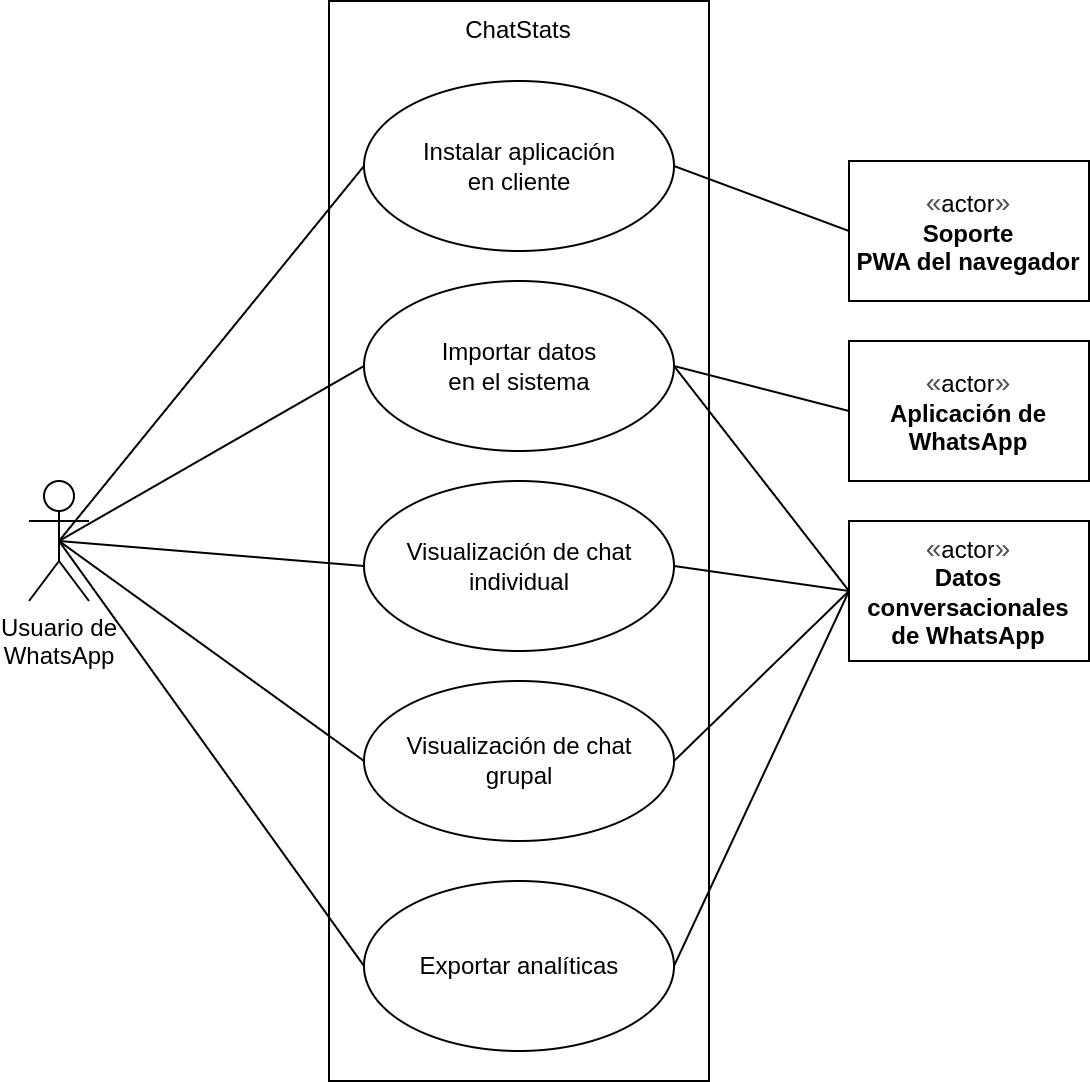
\includegraphics[width=0.8\textwidth]{img/uml.png}
	\caption{Diagrama \acrshort{uml}}
	\label{fig:chap3:uml}
\end{figure}

\begin{comment}
	Debería crear un caso de uso para chats individuales y otro para chats grupales?
	Debería diferenciar el caso de uso de PWA y web normal? (Por la integración con el SO)
	El actor es el archivo exportado y no WhatsApp.
	He cancelado el caso de uso de Telegram puesto que solo puede exportarse desde el ordenador y solo para algunos clientes.
\end{comment}

\section{Casos de uso}
\label{sec:use-cases}


\subsection{Actores del sistema}
\label{subsec:system-actors}

Usuario de WhatsApp o Telegram, datos conversacionales, aplicación de WhatsApp, aplicación de Telegram para escritorio y soporte PWA del navegador.

\paragraph{Usuario de WhatsApp o Telegram}\mbox{}\\

Se trata del usuario único en el que se centran nuestros casos de uso. Este es un usuario de WhatsApp o Telegram, ya que ChatStats es compatible con los archivos de chat exportados por estas aplicaciones.

\paragraph{Datos conversacionales}\mbox{}\\

Es el fichero de datos que nuestro sistema espera como entrada. En este caso de uso, se trata de un fichero de texto plano con todos los datos conversacionales exportados por la aplicación WhatsApp o Telegram para un chat individual o grupal, con o sin contenido multimedia.

\paragraph{Aplicación de WhatsApp}\mbox{}\\

Este actor constituye un sistema externo necesario para producir el actor anterior. Sin la aplicación de WhatsApp, ChatStats no tiene ninguna finalidad por sí solo.

\paragraph{Aplicación de Telegram para escritorio}\mbox{}\\

Este actor constituye un sistema externo necesario para producir los datos conversacionales. Sin la aplicación de Telegram para escritorio, ChatStats no tiene ninguna finalidad por sí solo.

\paragraph{Soporte \acrshort{pwa} del navegador}\mbox{}\\

Los navegadores con soporte para \acrfull{pwa} permiten instalar aplicaciones web, mejorando la integración con el sistema operativo.

\subsection{Instalar aplicación en el cliente}

\paragraph{Nombre del caso de uso} Instalar aplicación en el cliente.
\paragraph{Actores} Usuario de WhatsApp o Telegram, soporte \acrshort{pwa} del navegador.
\paragraph{Resumen} El usuario de WhatsApp o Telegram podrá, si su navegador lo soporta, instalar la aplicación de ChatStats para facilitar el acceso a la misma desde su sistema operativo y ofrecer mayor integración con el mismo.
\paragraph{Secuencia de acciones}\mbox{}\\

\begin{enumerate}
	\item El usuario accede a la página principal de ChatStats.
	\item El navegador con soporte \acrshort{pwa} le ofrece la opción de instalar la aplicación.
	\item El usuario instala la aplicación obteniendo un acceso directo en el escritorio o en el cajón de aplicaciones del navegador.
\end{enumerate}

\subsection{Importar datos en el sistema}

\paragraph{Nombre del caso de uso} Importar datos en el sistema.
\paragraph{Actores} Usuario de WhatsApp o Telegram, aplicación de WhatsApp, aplicación de Telegram para escritorio, datos conversacionales.
\paragraph{Resumen} El usuario de WhatsApp o Telegram exporta un chat de WhatsApp o Telegram, individual o grupal. Posteriormente, el usuario accede a la aplicación, selecciona e importa el archivo de datos conversacionales de WhatsApp. Finalmente, confirma su selección.
\paragraph{Secuencia de acciones}\mbox{}\\

\begin{enumerate}
	\item El usuario de WhatsApp o Telegram exporta un chat individual o grupal.
	\item El usuario accede a la aplicación.
	\item El usuario selecciona e importa el archivo de datos conversacionales exportado anteriormente.
	\item El usuario observa y confirma la selección.
\end{enumerate}

\subsection{Visualización de chat individual}

\paragraph{Nombre del caso de uso} Visualización de chat individual.
\paragraph{Actores} Usuario de WhatsApp o Telegram, datos conversacionales.
\paragraph{Resumen} El usuario puede observar, analizar e interactuar con las gráficas y estadísticas calculadas para chats individuales.
\paragraph{Secuencia de acciones}\mbox{}\\

\begin{enumerate}
	\item El usuario de WhatsApp o Telegram inicia el cálculo de estadísticas desde la aplicación.
	\item El usuario puede ver el número de mensajes enviado por ambas partes, así como el número de caracteres.
	\item El usuario puede ver la media de palabras y caracteres por mensaje.
	\item El usuario puede ver quién contesta más rápido los mensajes, así como el tiempo medio de respuesta.
	\item El usuario puede ver quién comienza normalmente las conversaciones, así como cuántas conversaciones ha comenzado cada uno.
	\item En caso de haber exportado el contenido multimedia, el usuario puede ver el número de fotos, vídeos, audios y pegatinas enviadas por ambas partes.
	\item El usuario puede ver tres distribuciones de mensajes: distribución de mensajes por mes, distribución de la media por día de la semana y distribución de la media de mensajes por hora del día.
	\item El usuario puede ver las palabras más utilizadas, así como los emoticonos.
\end{enumerate}

\paragraph{Condiciones previas} El usuario debe haber realizado anteriormente la exportación de un chat individual con o sin contenido multimedia desde la aplicación de WhatsApp o Telegram. También debe haber realizado la importación de datos en el sistema.

\subsection{Visualización de chat grupal}

\paragraph{Nombre del caso de uso} Visualización de chat grupal.
\paragraph{Actores} Usuario de WhatsApp o Telegram, datos conversacionales.
\paragraph{Resumen} El usuario puede observar, analizar e interactuar con las gráficas y estadísticas calculadas para chats grupales.
\paragraph{Secuencia de acciones}\mbox{}\\

\begin{enumerate}
	\item El usuario de WhatsApp o Telegram inicia el cálculo de estadísticas desde la aplicación.
	\item El usuario puede ver el número de mensajes enviado por cada persona, así como el número de caracteres.
	\item El usuario puede ver la media de palabras y caracteres por mensaje.
	\item El usuario puede ver quién contesta más rápido los mensajes, así como el tiempo medio de respuesta.
	\item El usuario puede ver quién comienza normalmente las conversaciones, así como cuántas conversaciones ha comenzado cada uno.
	\item En caso de haber exportado el contenido multimedia, el usuario puede ver el número de fotos, vídeos, audios y pegatinas enviadas por cada usuario.
	\item El usuario puede ver tres distribuciones de mensajes: distribución de mensajes por mes, distribución de la media por día de la semana y distribución de la media de mensajes por hora del día.
	\item El usuario puede ver las palabras más utilizadas, así como los emoticonos.
\end{enumerate}

\paragraph{Condiciones previas} El usuario debe haber realizado anteriormente la exportación de un chat grupal con o sin contenido multimedia desde la aplicación de WhatsApp o Telegram. También debe haber realizado la importación de datos en el sistema.

\subsection{Exportar analíticas}

\paragraph{Nombre del caso de uso} Exportar analíticas.
\paragraph{Actores} Usuario de WhatsApp o Telegram, datos conversacionales.
\paragraph{Resumen} El usuario puede exportar sus analíticas en un fichero, así como exportar una imagen para compartir las visualizaciones obtenidas.
\paragraph{Secuencia de acciones}\mbox{}\\

\begin{enumerate}
	\item El usuario de WhatsApp o Telegram desciende en la página de visualización.
	\item El usuario selecciona la opción de exportar o compartir.
	\item El usuario puede compartir la imagen de las visualizaciones obtenidas o guardar el archivo de los estadísticos calculados.
\end{enumerate}

\paragraph{Condiciones previas} El usuario debe haber realizado anteriormente la exportación de un chat grupal con o sin contenido multimedia desde la aplicación de WhatsApp o Telegram. También debe haber realizado la importación de datos en el sistema y el cálculo de las estadísticas para la visualización del chat.



\section{Especificación suplementaria}
\label{subsect:suplementary-specification}


\subsection{Reglas de dominio}

\begin{itemize}
	\item \textbf{Legales:} Cumplimiento de la Ley General de Protección de Datos Europea.
\end{itemize}

\begin{comment}
	No tenemos más reglas de dominio porque no tenemos requisitos o restricciones específicas a la industria o dominio de trabajo de nuestro caso de uso.
\end{comment}


\subsection{Requisitos no funcionales}

\begin{itemize}
	\item \textbf{Operación:} Interfaz de Usuario para navegador web, smartphone y tablet.
	
	\item \textbf{Seguridad:} Los datos no deben ser enviados a ningún servidor externo sin la autorización previa del usuario. Estos datos, además, no deben ser almacenados de manera temporal o permanente en ningún servidor. Todas las conexiones entre cliente y servidor deben estar cifradas con SSL.
	
	\item \textbf{Portabilidad:} La aplicación podrá ejecutarse en los navegadores: Chrome, Firefox, Edge y Safari; siendo compatible con \acrshort{pwa} en los navegadores que lo soporten.
	
	\item \textbf{Rendimiento:} El sistema debe ser capaz de analizar conversaciones de varios años sin aumentar drásticamente el tiempo de espera.
	
	\item \textbf{De implementación:} El código ha de ser libre bajo la licencia \acrfull{gplv3}.
\end{itemize}

\subsection{Restricciones}

\begin{itemize}
	\item \textbf{De interfaz:} uso de archivos \textit{txt} y \textit{zip} para importar los chats exportados desde la aplicación WhatsApp, puesto que únicamente exporta en estos dos formatos. Uso de archivos \textit{JSON} para importar los chats exportados desde la aplicación de Telegram para escritorio.
\end{itemize}










